\documentclass[11pt,a4paper]{book}
\usepackage[latin1]{inputenc}
\usepackage{amsmath}
\usepackage{amsfonts}
\usepackage{amssymb}
\usepackage{graphicx}
\usepackage{color}
\usepackage{geometry}
\usepackage{subcaption}
\usepackage{rotating}
\usepackage[dvipsnames]{xcolor}

\usepackage{doi}
%\usepackage[style=trad-plain]{biblatex}
\usepackage[backend=bibtex, sorting=none, style=numeric-comp]{biblatex}
\addbibresource{report.bib}
\DeclareDatamodelFields[type=field,datatype=literal]{mynote}
\usepackage{xpatch}
\xapptobibmacro{finentry}{\par\printfield{mynote}}{}{}


%\usepackage{lineno}
%\linenumbers

\newcommand{\pTvec}{\mathbf{p}_\mathrm{T}}
\newcommand{\qTvec}{\mathbf{q}_\mathrm{T}}
\newcommand{\qT}{q_\mathrm{T}}
\newcommand{\pTell}[1]{\mathbf{p}_\mathrm{T}^{\ell#1}}
\newcommand{\pTmiss}{\mathbf{p}_\mathrm{T}^\mathrm{miss}}

\usepackage{afterpage}
\newcommand\blankpage{%
	\null
	\thispagestyle{empty}%
	\addtocounter{page}{-1}%
	\newpage}

\begin{document}
\begin{titlepage}
	\begin{center}
		\vspace*{1cm}
		
		
\noindent
\begin{minipage}[t][][b]{.5\textwidth}
	\raggedright
	\color{NavyBlue}{
Technischen Universit\"{a}t M\"{u}nchen} \newline
\color{NavyBlue}{Fakult\"{a}t f\"{u}r  Physik}
\end{minipage}% <---------------- Note the use of "%"
\begin{minipage}[t][][b]{.5\textwidth}
	\raggedleft
	\includegraphics[width=0.2\linewidth]{figs/TUM}
\end{minipage}

	\vspace{2cm}
		\Large
		\textbf{Habilitation Thesis}
		
		\vspace{0.5cm}
		\Huge
		Search for Supersymmetry with the ATLAS detector at the LHC
		
		\vspace{1.5cm}
		\LARGE
		\textbf{Zinonas Zinonos}
		\vfill
		
		\begin{figure}[h]
			\centering
			\includegraphics[width=0.4\linewidth]{figs/front2}
		\end{figure}
		
		
		\vfill
		
		
		M\"{u}nchen, 2019
		
		\vspace{0.8cm}


%

		
	\end{center}
\end{titlepage}
\shipout\null
\shipout\null

\vspace*{\fill}
\noindent
Habilitation Thesis "Search for Supersymmetry with the ATLAS detector at the LHC".\newline

\noindent
Experimental High Energy and Particle Physics.\newline

\noindent
Max-Planck-Institut f\"{u}r Physik \& Technischen Universit\"{a}t M\"{u}nchen.\newline

\noindent
M\"{u}nchen, 2017-2019.\newline

\noindent
Defended on December 12, 2019.\newline

\noindent
Submitted in March, 2020.


\vspace{1cm}
\noindent
Mentoring committee:
\begin{itemize}
	\item	Prof. Dr. Hubert Kroha (Max-Planck-Institut f\"{u}r Physik, M\"{u}nchen, \textbf{Chair})
	\item	Prof. Dr. Stephan Paul (Technischen Universit\"{a}t M\"{u}nchen, \textbf{Member})
	\item 	Prof. Dr. Gregor Herten (Universit\"{a}t Freiburg, \textbf{Member})
\end{itemize}
%	\addcontentsline{toc}{section}{Acknowledgements}
\newpage


\section*{Acknowledgements}

First and foremost, I would like to express my sincere gratitude to my advisor Prof. Dr. Hubert Kroha (Max-Planck-Institut f\"{u}r Physik, M\"{u}nchen) for the continuous support on my habilitation project and related research as well as for his professionalism, motivation, and immense scientific knowledge. His insightful guidance and encouragement helped me in all the time of research and completion of this effort. I could not have imagined having a better advisor and mentor for my Habilitation.

Besides my advisor, I would like to express my gratitude to the rest of my Habilitation Committee:  Prof. Dr. Stephan Paul (Technischen Universit\"{a}t M\"{u}nchen, chairman of the committee) and Prof. Dr. Gregor Herten (Universit\"{a}t Freiburg), who provided me extensive guidance to achieve the scientific goals of this thesis. Also, I am grateful to all colleagues with whom I have had the pleasure to work during this and other related projects.

A very special gratitude goes to Prof. Dr. Siegfried Bethke, director at the Max Planck Institute for Physics in Munich, for encouraging and supporting me to pursue the habilitation program.

Most importantly, I am deeply indebted  to my loving, caring and supportive wife, Louiza, and my three wonderful daughters, Marina, Arsenia and Akylina, who endlessly provide me unending inspiration.

\clearpage
\tableofcontents

\chapter{Introduction}

\section{Motivation for Supersymmetry}

For several decades, particle physicists having been trying to better understand Nature at the smallest distances by colliding particles at the highest energies. While the Standard Model (SM) of particle physics has successfully explained most of the results that have arisen from experiments, many phenomena remain baffling. 

Supersymmetry, commonly abbreviated as SUSY, is one of the most appealing extensions of the  SM.  It is a generalization of the space-time symmetries of quantum field theory that proposes a relationship between two basic classes of elementary particles: bosons, which live in an integer-valued angular momentum eigenstate (spin), and fermions, which have a half-integer spin. Each particle from one group would have an associated particle in the other, which is known as its \textit{superpartner}, the spin of which differs by a half-integer. 


There are numerous phenomenological motivations for SUSY close to the electroweak scale, as well as technical motivations for this theory at any energy scale.

First, SUSY provides a framework for the unification of particle physics and
gravity~\cite{Martin:1997ns, nath_2016, Weinberg:2000cr}
at the Planck energy scale, $M_P \sim 10^{19}~\text{GeV}$, where the gravitational interactions become comparable in magnitude to the gauge interactions. Moreover, SUSY can provide an explanation of the large hierarchy between the energy scale that characterizes electroweak symmetry breaking, $M_\text{EW} \sim 100~\text{GeV}$, and the Planck scale~\cite{Witten:1981nf, DIMOPOULOS1981150, Sakai1981, SUSSKIND1984181}.
The stability of this large gauge hierarchy with respect to radiative
quantum corrections is not possible to maintain in the  SM without an
unnatural fine-tuning of the parameters of the fundamental theory at the Planck scale. 
More specifically, in a theory such as the  SM with an elementary scalar field of mass $m$ and interaction strength $\lambda$ (e.g. the quartic scalar self-coupling; the square of a gauge coupling or the square of a Yukawa coupling), the stability with respect to quantum corrections requires the existence of an
energy cutoff roughly of order $\sqrt{ (4\pi)^2/\lambda}\;m$ beyond which new physics must enter~\cite{PhysRev.56.72}.
A significantly larger energy cutoff would require an unnatural fine-tuning of parameters
that govern the low-energy theory. Applying this argument to the  SM leads
to an expectation of new physics at the TeV scale.
In a supersymmetric extension of the  SM, thereby, it is possible to maintain
the gauge hierarchy while providing a natural framework for elementary scalar fields.

Second, the unification of the three  SM gauge couplings at a very high
energy close to the Planck scale is possible if new physics beyond the  SM
(which modifies the running of the gauge couplings above the electroweak scale) is
present. The minimal supersymmetric extension of the  SM (MSSM), where
superpartner masses lie below a few TeV, provides an example of successful gauge
coupling unification~\cite{Polonsky:2001pn}.

Third, the existence of dark matter (DM), which makes up approximately one quarter of the
energy density of the universe, cannot be explained within the  SM of particle
physics~\cite{Bertone:2004pz}.
Remarkably, a stable weakly-interacting massive particle (WIMP) whose
mass and interaction rate are governed by new physics associated with the TeV-scale
can be consistent with the observed density of dark matter, the so-called \textit{WIMP
miracle},. The lightest supersymmetric particle, if stable, is
a promising (although not the unique) candidate for the DM~\cite{PhysRevLett.48.223, ELLIS1984453, Steffen2009}.

\begin{figure}
 \centering
 \includegraphics[width=0.6\linewidth]{figs/gut}
 \caption{Two-loop renormalization group evolution of the
  inverse gauge couplings $\alpha^{-1}_{a}(Q)\,\, a=1;\,2,\;3$ as a function of the energy scale $Q$ in the  SM (dashed
  lines) and the MSSM (solid lines). Unlike the SM, the MSSM includes just the
  right particle content to ensure that the gauge couplings can unify, at a scale $M_U \sim 1.5 \times 10^{16}~\text{GeV}$. Adapted from Ref.~\cite{Martin:1997ns}.}
 \label{fig:gut}
\end{figure}


If SUSY were an exact symmetry of nature, then particles and their superpartners would be degenerate in mass. Since superpartners have not (yet) been observed by experiments, SUSY must be a broken symmetry. Despite the break down of SUSY, the stability of the gauge hierarchy can still be maintained if the
SUSY breaking is soft~\cite{Girardello:1981wz, Jack:1999ud}, and the corresponding SUSY-breaking mass parameters are no larger than a few TeV. This, in fact, makes the search of SUSY plausible at modern collider experiments since it lies within the energy reach, for example, the Large Hadron Colllider (LHC) at CERN located in Geneva.

\section{Minimal Supersymmetric  Standard Model}
In its minimal realization, the MSSM,  
SUSY postulates the existence of a new bosonic (fermionic) partner for each fundamental  SM fermion (boson), as well as an additional Higgs doublet. 
More specifically, electroweakly interacting supersymmetric particles are charginos, neutralinos, sleptons, sneutrinos and squarks. Charginos ($\tilde{\chi}^\pm$) and neutralinos ($\tilde{\chi}^0$) are the mass eigenstates formed by linear combinations of the superpartners of the charged and neutral Higgs bosons and of the electroweak gauge bosons. Strongly interacting superpartners are the squarks ($\tilde{q}$) and gluinos ($\tilde{g}$). 

\begin{figure}
 \centering
 \includegraphics[width=0.85\linewidth]{figs/mssm}
 \caption{Particle content of the Minimal Supersymmetric  SM theory.}
 \label{fig:mssm}
\end{figure}

The minimal supersymmetric extension of the  SM also consists of the fields of the two-Higgs-doublet extension of the  SM and the corresponding superpartners.
After electroweak symmetry breaking, five Higgs bosons arise, of
which two are charged. The supersymmetric partners of the Higgs doublets are known
as "higgsinos".
The enlarged Higgs sector of the MSSM constitutes the minimal structure needed to guarantee
the cancellation of gauge anomalies~\cite{PhysRevD.6.429}
generated by the higgsino superpartners that can appear as internal lines in triangle diagrams with three external electroweak gauge bosons. 
Moreover, without a second Higgs doublet, one cannot generate mass for both
"up"-type and "down"-type quarks, and charged leptons in a way consistent with the
underlying SUSY~\cite{Fayet:1974pd, Gunion:1984yn}.

The fact that such particles are not yet observed leads to the conclusion that, if SUSY is realized, it is a broken symmetry. A description of SUSY in the form of an effective Lagrangian
with only "soft" SUSY breaking terms and SUSY masses at the TeV scale maintains
cancellation of quadratic divergences in particle physics models

\section{R-Parity}
In the absence of a protective symmetry, SUSY processes violating the lepton ($L$) and baryon ($B$) quantum numbers result in proton decay at a rate that is in conflict with the experimental constraints on its lifetime. This conflict can be avoided by imposing a $B-L$  conservation requirement on the supersymmetric Lagrangian when defining the MSSM.  As a consequence of the $B-L$ symmetry, the MSSM possesses a multiplicative R-parity invariance, which is defined as
\begin{equation}
R = (-1)^{3(B-L)+2S}
\end{equation}
for a particle of spin S~\cite{FARRAR1978575}. This implies that all the particles of the  SM have even R-parity, whereas the corresponding
superpartners have odd R-parity. 
\begin{figure}[htbp]
	\centering
	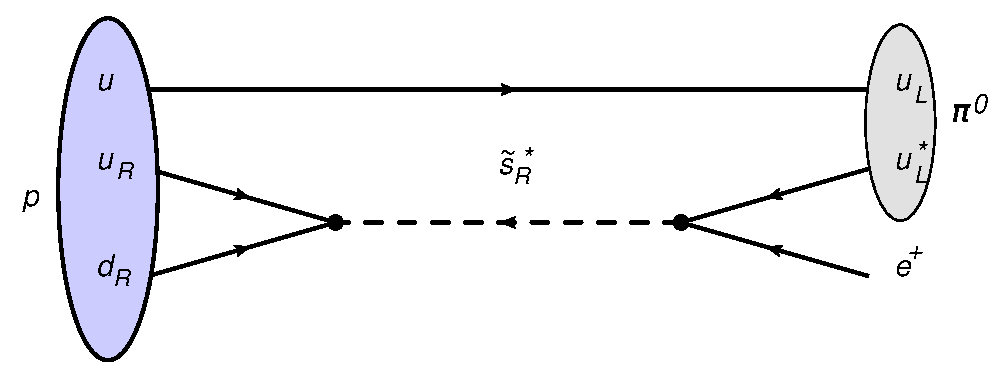
\includegraphics[width=0.5\linewidth]{figs/p-decay}
	\caption{Proton decay into a positron and a neutral pion.}
	\label{fig:p-decay}
\end{figure}


The conservation of R-parity in scattering and decay processes has a critical impact on supersymmetric phenomenology. For example, any initial state in a scattering experiment will involve ordinary (R-even) particles. Consequently, it follows that supersymmetric particles must be produced in pairs. 
In general, these particles are highly unstable and decay into lighter states.
R-parity invariance also implies that the lightest supersymmetric particle (LSP) is
absolutely stable, and must eventually be produced at the end of a decay chain initiated
by the decay of a heavy unstable supersymmetric particle.
In order to be consistent with cosmological constraints, a stable LSP is certainly
electrically and color neutral~\cite{ELLIS1984453}. Therefore, the LSP in an R-parity-conserving (RPC) theory is weakly interacting with ordinary matter, i.e., it behaves like a stable heavy neutrino and will escape collider detectors without being directly observed. Thus, the canonical signature for conventional RPC supersymmetric theories is substantial missing (transverse) energy, due to the LSP escaping from any detection means. Finally, the stability of the LSP in RPC SUSY makes it a promising candidate for dark matter.

If R-parity is violated, new lagrangian terms parameterized by $\lambda_{ijk}$,  $\lambda_{ijk}^\prime$  and  $\lambda_{ijk}^{\prime\prime}$ appear in the superpotential, where $ijk$ are particle generation indices. 
\begin{equation}
W =  \lambda_{ijk} \mathrm{L}_i  \mathrm{L}_j   \bar{\mathrm{E}}_k
+  \lambda_{ijk}^\prime  \mathrm{Q}_i  \mathrm{L}_j   \bar{\mathrm{D}}_k
+  \lambda_{ijk}^{\prime\prime}  \bar{\mathrm{U}}_i  \bar{\mathrm{D}}_j   \bar{\mathrm{D}}_k
+ m_i \mathrm{L}_i  \mathrm{H}_u
\end{equation}
where Q, U, D, L, E  are the matter superfields and $\mathrm{H}_{u,d}$ are the up and down type Higgs superfields.
The $\lambda$-type couplings appear between lepton superfields only, $\lambda^{\prime}$-type are between quark superfields only, and $\lambda^{\prime\prime}$-type couplings
connect the two. R-parity violation (RPV) implies lepton and/or baryon number violation. 
In this case, the lightest neutralino can decay even if it is the LSP. If the decay involves a non-zero $\lambda$ coupling, the final state will be a multi-lepton one.
Searches for events with four or more isolated charged
leptons by the ATLAS~\cite{ATLAS-CONF-2015-018, ATLAS-CONF-2016-075, Aaboud:2018zeb} 
and CMS~\cite{CMS-PAS-SUS-13-010} 
experiments are interpreted in such models. The search of multi-lepton final states and interpretation in SUSY RPV models is subject of this thesis.
With very small coupling values, the neutralino would be long-lived, leading to lepton pairs with a
displaced vertex, which have also been searched for~\cite{PhysRevD.92.072004, CMS:2015pca}.

\section{Phenomenology of Supersymmetry}
The phenomenology of SUSY is to a large extent determined by the SUSY breaking mechanism and the SUSY breaking scale. This determines the SUSY particle masses, the mass hierarchy, the field contents of physical particles, and their decay modes. 
In addition, phenomenology crucially depends on whether the multiplicative quantum number of R-parity is conserved or violated. In most cases, supersymmetric events are characterized by a high multiplicity of final state particles and a large amount of missing transverse energy due to the undetected LSP and possible production of neutrinos.

Since the mechanism by which SUSY is broken is unknown, a general approach to
SUSY via the most general soft SUSY breaking Lagrangian adds a significant number
of new free parameters. For the MSSM, these comprise 105 new parameters. A
phenomenological analysis of SUSY searches leaving all these parameters free is not
feasible. For the practical interpretation of SUSY searches at colliders, several approaches are taken to reduce the number of free parameters. The most common approach is to assume a SUSY breaking mechanism and lower the number of free parameters through the assumption of additional constraints, such the R-parity conservation or not, the particle masses and decay branching ratios.

At the LHC, most searching approaches are developed to increase the sensitivity to pair production of heavy sparticles with TeV-scale masses focusing on the kinematics of their decays, and to further suppress the background from  SM processes.

Selection variables designed to separate the SUSY signal from the SM backgrounds typically include $H_\mathrm{T}$, $E_\mathrm{T}^\text{miss}$, and $m_\text{eff}$. The reconstructed quantities  $H_\mathrm{T}$ and $E_\mathrm{T}^\text{miss}$
refer to the measured transverse energy and missing transverse momentum in the event, respectively. They are defined as the scalar sum of the transverse particle momenta or calorimeter clusters transverse energies measured in the event ($H_\mathrm{T}$), or the negative vector sum of transverse momenta of reconstructed objects like jets and leptons in the event ($E_\mathrm{T}^\text{miss}$). The event observable  $m_\text{eff}$ is referred to as the effective mass of the event and is defined as the sum of $H_\mathrm{T}$ and $E_\mathrm{T}^\text{miss}$. The peak of the  $m_\text{eff}$  distribution for SUSY signal events correlates with the SUSY mass scale, in particular with the mass difference between the primary produced SUSY particle and the LSP, whereas the  SM backgrounds
typically dominate at low $m_\text{eff}$ values.  Additional reduction of multijet backgrounds can be achieved by requiring isolated leptons or photons in the final states.

Recently, alternative approaches have been developed to increase the sensitivity
to pair production of heavy sparticles with TeV-scale masses focusing on the kinematics
of their decays, and to further suppress the background from multijet production.
Prominent examples of these new approaches are searches using the $\alpha_T$ variable~\cite{PhysRevLett.101.221803, Chatrchyan:2013mys},
\textit{razor} variables~\cite{Chatrchyan:2012lia}, \textit{stransverse mass}  ($m_{\mathrm{T}2}$)~\cite{Lester:1999tx},
and contransverse mass ($m_{\mathrm{CT}}$)~\cite{Tovey:2008ui}. 
In particular, a lower bound on the stransverse mass can be imposed in event selections to reduce contributions from $t\bar{t}$ and $WW$ events.
The $m_{\mathrm{T}2}$ variable is defined as:
\begin{equation}\label{eq:mt2}
m_{\mathrm{T}2} = \min_{\mathbf{q}_\mathrm{T}}\left[\max\left(m_{{\mathrm T}}^{(1)}(\mathbf{p}_{\mathrm{T}}^{(1)},\, \mathbf{q}_\mathrm{T}),m_{\mathrm T}^{(2)} (\mathbf{p}_{\mathrm{T}}^{(2)},\mathbf{E}_\mathrm{T}^\mathrm{miss}-\mathbf{q}_\mathrm{T})\right)\right],
\end{equation}
where $\mathbf{p}_{\mathrm{T}}^{(i)}, \; i =1,\;2$ are the transverse momenta of a reconstructed particle pair, and $\qTvec$ is the transverse momentum vector that minimizes the larger of the
two transverse masses $m_{{\mathrm T}}^{(i)},\, \; i =1,\;2$.
The latter masses are defined by
\begin{equation}
m_{{\mathrm T}}(\pTvec,\, \mathbf{q}_\mathrm{T}) = \sqrt{2(p_\mathrm{T}\qT-\pTvec\cdot \mathbf{q}_\mathrm{T})}\; .
\end{equation}
For $t\bar{t}$  and $WW$ events, in which two $W$ bosons decay leptonically and $\mathbf{E}_\mathrm{T}^\mathrm{miss}$
is the sum of the transverse momenta of the two neutrinos, the $m_{\mathrm{T}2}$ distribution has a kinematic end-point at the $W$ mass. For large mass differences between the staus and the lightest neutralino, the $m_{\mathrm{T}2}$ distribution for signal events extends significantly beyond this end-point.


Furthermore, the topological event reconstruction methods have expanded with the \textit{superrazor}~\cite{Buckley:2013kua}
and \textit{recursive jigsaw reconstruction}~\cite{PhysRevD.96.112007} techniques. 
Finally, the searches including massive SUSY particles attempt to identify their decay into top quarks or vector bosons, which are themselves unstable. If these are produced with a significant boost, jets(tau lepton) from their decay will typically overlap, and such topologies are searched for with jet(tau lepton)-\textit{substructure} techniques~\cite{PhysRevLett.100.242001}.

\section{Experimental Search Program for SUSY}
Searches for SUSY and new physics in general were part of the physics program of large collider experiments, such as the LEP electron-positron collider at CERN, the Tevatron proton-antiproton collider at Fermilab, the HERA electron-proton collider at DESY, and the LHC proton-proton ($pp$) collider at CERN.

Searches for new physics at $e^+e^-$ colliders benefit from the clean experimental
environment and the fact that momentum balance can be measured not only in the plane
transverse to the beam, but also in the direction along the beam pipe, defined as the longitudinal direction. Searches at LEP are dominated by the data
samples taken at the highest center-of-mass energies.
On the other hand, proton-(anti)proton colliders produce interactions at higher center-of-mass energies than those available at LEP, and cross sections of QCD-mediated processes are larger, which is reflected in the higher sensitivity for SUSY particles carrying color charge: squarks and gluinos. Large background contributions from  SM processes, nonetheless, pose challenges to data acquisition and analysis. Such backgrounds are dominated by QCD multijet production processes, the top quark production, as well as jet production in association with vector gauge bosons. The proton momentum is shared between its parton constituents, and in each collision only a fraction
of the total center-of-mass energy is available in the hard parton-parton scattering.
Since the parton momenta in the longitudinal direction are not known on an event-by-event
basis, use of momentum conservation constraints in an analysis is restricted to the
transverse plane, leading to the definition of transverse variables, such as the missing
transverse energy $E_\mathrm{T}^\text{miss}$, and the transverse mass $m_\mathrm{T}$.

Today, there is no evidence to show whether or not SUSY is correct, or what other extensions to current supersymmetric models might be more accurate. Despite this, SUSY is being supported by physicists since it remains the most complete theory to describe possible phenomena beyond the SM. 
%
Low-energy data from flavor physics experiments, high-precision electroweak
observables as well as astrophysical data impose strong constraints on the allowed
SUSY parameter space. 
Recent examples of such data include measurements of the rare B-meson decay 
$B_s \to \mu^+ \mu^-$~\cite{Oyanguren:2018huo, PhysRevLett.118.191801}, measurements of the anomalous magnetic moment
of the muon~\cite{Czarnecki:2000id}, and accurate determinations of the cosmological dark matter relic density constraint~\cite{Ade:2015xua}.

These indirect constraints are often more sensitive to higher SUSY mass scales than
experiments searching for direct sparticle production at colliders, but the interpretation of
these results is often strongly model dependent.
%
On the other hand, direct confirmation would entail production of superpartners in collider experiments, such as the LHC. 
Direct searches for sparticle production at collider experiments are less subject to interpretation ambiguities and therefore they play a crucial role in the search for SUSY.

The first runs of the LHC found no previously-unknown particles other than Higgs boson with a mass around 125 GeV, which was already suspected to exist as part of the  SM. With the discovery of the Higgs boson, further constraints were imposed on a plethora of SUSY models~\cite{PhysRevD.98.030001}.


\section{Scope of Thesis}

This habilitation thesis attempts to cover searches from the electroweak sector of SUSY, mostly involving leptons in the final state. The electroweak processes are characterized by a very small production cross-section, at minimum one order of magnitude less than those processes involving the strong force, as presented by Figure~\ref{fig:xsec1}. Due to exactly the colored production of gluinos and squarks, the SUSY partners of gluons and quarks, hadron collider experiments are able to set much tighter mass limits.
\begin{figure}[htbp]
 \centering
 \includegraphics[width=0.7\linewidth]{figs/xsec1}
 \caption{Cross sections for pair production of different SUSY production modes as a
  function of the sparticle mass at the LHC for a center-of-mass energy of 13~TeV.
  The cross section of pair production of electroweak gauginos at the LHC, for masses of several hundreds of GeV, is at least two orders of magnitude smaller than for colored SUSY particles (e.g. top squark pair production). Adapted from Ref.~\cite{susy:xsec}.
 }
 \label{fig:xsec1}
\end{figure}
Despite this fact, the search for SUSY in electroweak scenarios is also feasible due the distinct signal signatures in the event final state which suppress significantly the SM background sources.
For example, the search of multileptonic final states requires the presence many leptons in the event, and the search of direct production of tau sleptons require high values of the $m_\text{eff}$ observable. Both selection requirements reduce significantly the SM processes that mimic these SUSY signal events.
The search of these SUSY scenarios consist the main topic of this thesis, which presents the methodology and discusses the main results. Since none of the searches performed so far have shown significant excess above the  SM background prediction, the interpretation of the presented results is focused on showing exclusion limits on the SUSY parameter space.

In the following, the ATLAS detector at the LHC is shortly described. Then, the main ingredients of the analysis structure and result interpretation are presented, as well as the conclusions of each search. Whereas necessary, the assumptions that have entered the limits when quoting interpretations from simplified models will be explicitly pointed out. The papers accepted for publication or already published in electronic journals are enclosed in the Appendix~\ref{ch:app}.


\chapter{ATLAS Detector}
The ATLAS detector~\cite{ATLAS_2008}, shown in Figure~\ref{fig:atlas}, is a multipurpose particle detector with a forward-backward symmetric cylindrical
geometry and nearly $4\pi$ coverage in solid angle.
\begin{figure}[htbp]
 \centering
 \includegraphics[width=0.9\linewidth]{figs/atlas}
 \caption{Cutaway drawing of the ATLAS detector showing its main detection components.}
 \label{fig:atlas}
\end{figure}
The entire detector weighs approximately 7,000 tons, and is 44 m long and 25 m in diameter. It is situated in an underground cavern at a depth of 100 m, where it surrounds one of the collision points around the 27-km-long LHC ring. The first $pp$ collisions at the LHC were recorded in 2009, and since then collider has operated at different center-of-mass-energies, namely 7, 8 and 13~TeV.

\section{Coordinate System}
ATLAS uses a right-handed coordinate system with its origin at the nominal interaction point (IP) in the center of the detector and the z-axis along the beam pipe. The x-axis points from the IP to the center of the LHC ring, and the y-axis points upward. 
Cylindrical coordinates $(r,\, \phi)$ are used in the transverse plane, $\phi$ being the azimuthal angle around the z-axis. Pseudorapidity, $\eta$, is defined in terms of the polar angle $\theta$ as $\eta = - \ln \tan(\theta/2)$. Rapidity is defined as $y = 0.5 \ln (E + p_z )/(E - p_z )$
where $E$ denotes the energy and $p_z$ is the component of the momentum along the beam direction.

\section{Inner Detector}
The inner tracking detector (ID) consists of silicon pixel detector and semiconductor tracker (SCT) detectors covering the pseudorapidity region $|\eta| < 2.5$. These systems are surrounded by a transition
radiation tracker (TRT), which enhances electron identification in the region $|\eta| < 2.0$. 
Before LHC Run 2, a new innermost pixel layer, the insertable B-layer~\cite{CERN-LHCC-2012-009}, was inserted at a mean sensor radius of $3.3$~cm. 
\begin{figure}[thbp]
 \centering
 \includegraphics[width=0.7\linewidth]{figs/id}
 \caption{Cut-away image of the ATLAS Inner Detector.}
 \label{fig:id}
\end{figure}
The ID is surrounded by a thin superconducting solenoid providing an axial 2~T magnetic field.

\section{Calorimeters}
A fine granularity lead/liquid-argon (LAr) electromagnetic (EM) calorimeter, covering $|\eta| < 3.2$, is used to reconstruct electrons and photons.
A steel/scintillator tile calorimeter provides coverage for hadronic showers in the central pseudorapidity range ($|\eta| < 1.7$).

The endcaps ($1.5 < |\eta| < 3.2$) of the hadronic calorimeter have LAr active layers with either copper
or tungsten as the absorber material. The forward region ($3.1 < |\eta| < 4.9$) is instrumented with a LAr
calorimeter for both the EM and hadronic measurements. 

\section{Muon Spectrometer}

The ATLAS muon spectrometer (MS) is cylindrical, 22~m in diameter and 45~m in length, surrounding the
calorimeters with an acceptance coverage of $2\pi$ in azimuth and $\pm 2.7$ in pseudorapidity.
It is designed to detect muons in the pseudorapidity region
up to $|\eta| = 2.7$, and to provide momentum measurements with a relative resolution $\delta p /p$ better than 3\% over a wide  $p_T$ range and up to 10\% at $p_T \simeq 1$~TeV~\cite{Aad:2016jkr}. 

The MS consists of one barrel ($|\eta| < 1.05$) and two endcap sections ($1.05 < |\eta| < 2.7$). 
A system of three large superconducting air-core toroidal magnets, each with eight coils, provides a magnetic field with a bending integral  $B \cdot dl$ of about $2.5~\mathrm{T}\cdot \mathrm{m}$ in the barrel and up to $6~\mathrm{T}\cdot \mathrm{m}$ in the endcaps. 
Resistive plate chambers (RPC, three doublet layers for $|\eta| < 1.05$) and thin gap chambers
(TGC, one triplet layer followed by two doublets for $1.0 < |\eta| < 2.4$) provide triggering capability to the detector as well as $(\eta,\; \phi)$ position measurements with typical spatial resolution of $5 - 10~\text{mm}$. 
A precise momentum measurement for muons with pseudorapidity up to $|\eta| = 2.7$ is provided by three layers of monitored drift tube chambers (MDT), with each chamber providing six to eight $\eta$ measurements along the muon trajectory. 
For $|\eta| > 2$, the inner layer is instrumented with a quadruplet of cathode strip chambers (CSC) instead of MDTs. 
The single-hit resolution in the bending plane for the MDT and the CSC is about $80~\mu\mathrm{m}$ and $60~\mu\mathrm{m}$, respectively. 
The muon chambers are aligned with a precision between $30~\mu\mathrm{m}$ and $60~\mu\mathrm{m}$.


%
\begin{figure}[hbtp]
 \centering
 \includegraphics[width=0.45\linewidth]{figs/muons}
 \caption{Cross-sectional view of the ATLAS muon spectrometer.}
 \label{fig:muons}
\end{figure}
%


\section{Trigger System}
The ATLAS trigger system~\cite{Aaboud:2016leb} consists of a hardware-based level-1 (L1) trigger followed by a software-based high-level trigger (HLT). 

The L1 hardware trigger is constructed with custom-made electronics and runs with a fixed latency of $2.5~\mu\mathrm{s}$. It works on a subset of information from the calorimeter and muon detectors. The decision to keep the data from an event is made less than two-and-half microseconds after the event occurs, and the event is then retrieved from pipelined storage buffers. The L1 trigger reduces substantially the event rate from the LHC interaction rate of 40 MHz, and can save at most 100~k events per second for the HLT. 

The HLT software trigger-based trigger is assembled by a large farm of CPUs and serves to refine the analysis of the L1 trigger. In the HLT, offline-like reconstruction algorithms run in a large farm of  $\sim 40$k processor cores and a decision is formed typically within 300~ms. It conducts a very detailed analysis either by performing overall examination of the whole event for selected layers of the detector (for example calorimeters, trackers, muon detectors), or, by utilizing the data in smaller and isolated regions of the detector. About 1k events per second are selected by the HLT analysis and are fully assembled into an event record. These events are finally passed on to a data storage system for offline analysis.

\section{Luminosity}
A precise measurement of the integrated luminosity is a key component of the ATLAS physics program, in particular for cross-section measurements where it is often one of the leading sources of
uncertainty~\cite{ATLAS-CONF-2019-021}. The luminosity measurement is based on an absolute calibration of the primary luminosity-sensitive detectors in low-luminosity runs with specially-tailored LHC conditions using the van der Meer (vdM) method~\cite{GRAFSTROM201597}. 
The total uncertainties on the integrated luminosity measurements  for each individual year of data-taking range from 2.0 to 2.4\%, and are partially correlated between years.

Figures~\ref{fig:intlumivsyear} and \ref{fig:intlumivstimerun2dqall} presents the cumulative luminosity versus day delivered to ATLAS during stable beams and for high energy $pp$ collisions.
\begin{figure}
 \centering
 \includegraphics[width=0.75\linewidth]{figs/intlumivsyear}
 \caption{Delivered luminosity to ATLAS for $pp$ collisions versus time for years 2011-2018~\cite{lumi-atlas}.}
 \label{fig:intlumivsyear}
\end{figure}
After typical data-quality selections, the full Run 2 $pp$ data sample corresponds to an integrated luminosity of $139~\mathrm{fb}^{-1}$, with an uncertainty of 1.7\%.

\begin{figure}
	\centering
	\includegraphics[width=0.75\linewidth]{figs/intlumivstimeRun2DQall}
	\caption{Cumulative luminosity versus time delivered to ATLAS (green), recorded by ATLAS (yellow), and certified to be good quality data (blue) during stable beams for pp collisions at 13 TeV centre-of-mass energy in 2015-2018. }
	\label{fig:intlumivstimerun2dqall}
\end{figure}


\chapter{Searches and Methodology}


\section{Search for SUSY in multileptonic final states}


\subsection{Motivation}
Multileptonic final states consist a very attractive channel for the search for new physics at the LHC because the overwhelming hadronic background can be strongly suppressed. 
In RPV models, the lightest SUSY particle is unstable
and decays to SM particles, including charged leptons and neutrinos when violating L but not B. 
In RPC models, the LSP is stable and leptons can originate from unstable weakly interacting sparticles decaying into the LSP. 
Therefore, both the RPV and RPC SUSY scenarios can result in signatures with high lepton multiplicities and substantial missing transverse momentum.

Requiring a high multiplicity of isolated leptons (electrons and muons - including those originating from leptonic tau decays - and hadronically decaying taus), allows any new signature to be cleanly separated from the otherwise overwhelming hadron-rich background processes, typical of high-energy $pp$ collisions, even if its cross-section is small. 

More specifically, within this habilitation program, multiple searches for the production of charginos, neutralinos, sleptons and gluinos decaying to final states with at least four charged leptons are conducted. These searches exploit the complete $pp$ collision dataset delivered by the LHC at a center-of-mass energy of $\sqrt{s}=13$~TeV, and collected and reconstructed with the ATLAS detector. Particular emphasis is placed on the search for light higgsino particles. The exclusion of gluino and stop masses up to the TeV mass scale qualifies�now the light higgsinos to be discovered first at LHC, as motivated by naturalness. In General Gauge Mediated (GGM) SUSY models, the gravitino (supersymmetric particle of graviton) is nearly massless and is the LSP offering the possibility to study light higgsinos. Typical higgsino signal events are characterized by multiple charged leptons substantial MET, which is a distinct signature used to identify higgsino events. 

The search itself is optimized using several signal models but is generally model-independent using loose requirements on effective mass or missing transverse energy. 
Results are presented in terms of the number of events from new physics processes with a four charged lepton signature, and in particular in terms of RPC or RPV
simplified models with decays of the LSP to charged leptons.

%The analysis was published in 2018~\cite{Aaboud:2018zeb} and presented at the ICHEP2018 and SUSY2018 conferences.

\subsection{Scenarios}
Simplified models of RPV scenarios are considered, where the LSP is a bino-like neutralino ($\tilde{\chi}^0_1$) and decays via an RPV interaction. The LSP decay is described by the $\frac{1}{2} \lambda_{ijk}L_i L_j \bar{E}_k$ lepton-number-violating superpotential term, where $L_i$ and $E_i$ indicate the lepton SU(2)-doublet superfield and singlet superfield, respectively. Lepton generations are referred to by the indices $i$, $j$ and $k$ while $\lambda_{ijk}$ corresponds to nine Yukawa couplings which allow the decay of the LSP to every possible combination of charged lepton pairs. In this search, two extremes of the $\lambda_{ijk}$ RPV couplings are considered: $ L_1 L_2 \bar{E}_k\, (k=1,\,2)$ where only decays to electrons and muons are considered, and  $ L_i L_3 \bar{E}_3\, (i=1,\,2)$ where only decays to taus and either electrons or muons are included.

Three different RPV scenarios are searched in this thesis for the next-to-lightest-supersymmetric particle (NLSP) in the $ L_1 L_2 \bar{E}_k$ ($\lambda_{12k}$) and $ L_i L_3 \bar{E}_3$ ($\lambda_{i33}$): 
\begin{enumerate}
 \item Wino NLSP, where mass-degenerate wino-like charginos and neutralinos are produced in association;
 \item Slepton/sneutrino NLSP, where mass-degenerate left-handed sleptons and sneutrinos of all three generations are produced in association; and 
 \item Gluino NLSP, where the produced gluinos decay to the LSP while emitting a quark-antiquark pair each.
\end{enumerate}

These scenarios, as diagrammatically shown in Figure~\ref{fig:RPV_models},  result typically in signatures with high lepton multiplicities and substantially high values of the the effective mass observable, $m_\text{eff}$.
These features of the final state can be used to select signal events while suppressing the  SM background drastically.

\begin{figure}[htbp]
 \centering
 \begin{subfigure}[b]{0.35\textwidth}
  \includegraphics[width=\textwidth]{figs/fig_01a.pdf}
  \caption{Wino W/Z NLSP}
  \label{fig:fig_01a}
 \end{subfigure}
 ~ 
 \begin{subfigure}[b]{0.35\textwidth}
  \includegraphics[width=\textwidth]{figs/fig_01b.pdf}
  \caption{Wino W/h NLSP}
  \label{fig:fig_01b}
 \end{subfigure}
 \\
 \begin{subfigure}[b]{0.35\textwidth}
  \includegraphics[width=\textwidth]{figs/fig_01c.pdf}
  \caption{Slepton/sneutrino NLSP}
  \label{fig:fig_01c}
 \end{subfigure}
 %
 \begin{subfigure}[b]{0.35\textwidth}
  \includegraphics[width=\textwidth]{figs/fig_01d.pdf}
  \caption{Gluino NLSP}
  \label{fig:fig_01d}
 \end{subfigure}

 \caption{Diagrams of the processes in the SUSY RPV models considered in the analysis.}\label{fig:RPV_models}
\end{figure}


This analysis is also optimized to search RPC scenarios with light $\tilde{\chi}^0_1$, $\tilde{\chi}^0_2$, $\tilde{\chi}^\pm_1$ higgsino triplet states in the context of GGM, which predicts the gravitino ($\tilde{G}$, the fermionic superpartner of the graviton) nearly massless giving the opportunity to study light higgsinos (shown in Figure~\ref{fig:hino}). Light higgsinos are well motivated by naturalness~\cite{BARBIERI198863, deCarlos:1993rbr}.
\begin{figure}[htbp]
\centering
\includegraphics[width=0.4\linewidth]{figs/ggm}
\caption{Diagrams of the processes in the GGM higgsino models considered in the analysis.}
\label{fig:hino}
\end{figure}

Typically, the members of the higgsino triplet are close in mass its decays result in low-momentum decay products that are difficult to reconstruct efficiently. However, the decays of the higgsinos themselves to the LSP $\tilde{G}$ would lead to on-shell Z/h, and the decay products can be therefore efficiently reconstructed, as illustrated in Figure~\ref{fig:ggm}.
\begin{figure}[htbp]
 \centering
 \includegraphics[width=0.7\linewidth]{figs/hino}
 \caption{Chart illustrating the decay chain of the higgsino triplet $\tilde{\chi}^0_1$, $\tilde{\chi}^0_2$, $\tilde{\chi}^\pm_1$ to a nearly massless gravitino, $\tilde{G}$, LSP. The decays of the higgsinos to the LSP would lead to on-shell Z/h, and the decay products can be thus reconstructed. }
 \label{fig:ggm}
\end{figure}
In this search, simplified RPC models inspired by GGM are considered, where the only SUSY particles within reach of the LHC are an almost mass-degenerate higgsino triplet $\tilde{\chi}^0_1$, $\tilde{\chi}^0_2$, $\tilde{\chi}^\pm_1$ and a massless $\tilde{G}$. Finally, the $ \tilde{\chi}^0_1 \to Z \tilde{G}$ branching ratio is a free parameter of the GGM higgsino scenarios, and so offers an opportunity to study four-lepton signatures with one or more Z-boson candidates.


\subsection{Methodology}
Events are selected using single-lepton or dilepton triggers, where the trigger efficiencies are in the plateau
region above the offline $p_\mathrm{T}$ thresholds. The latter are typically a bit higher than the online ones. Dilepton triggers are used only when the leptons in the event fail $p_\mathrm{T}$-threshold requirements for the single-lepton triggers.

Events with four or more signal leptons ($\ell =e,\, \mu$ and hadronically decaying $\tau_\mathrm{had-vis}$) are selected and are classified according to the number of light signal leptons (L = e, $\mu$) and signal taus (T): at least four light leptons and exactly zero taus 4L0T, exactly three light leptons and at least one tau 3L1T, or exactly two light leptons and at least two taus 2L2T .

Events are further classified according to whether they are consistent with a leptonic Z boson decay or not. The Z-boson requirement selects events where any same-flavor LL pair combination with opposite electric charge (SFOS)  has an invariant mass close to the Z-boson mass, in the range $81.2-101.2$~GeV. A second Z candidate may be identified if a second SFOS LL pair is present and satisfies $61.2 < m(LL) < 101.2$~GeV.
To suppress radiative Z boson decays into four leptons (where a photon radiated from a $Z \to \ell \ell$ decay converts to a second SFOS lepton pair) the Z veto also considers combinations of any SFOS LL pair with an additional lepton (SFOS+L), or with a second SFOS LL pair (SFOS+SFOS), and rejects events where either the SFOS+L or SFOS+SFOS invariant mass lies in the range $81.2-101.2$~GeV.

%The missing transverse momentum, $E_\mathrm{T}^\mathrm{miss}$, is the magnitude of the negative vector sum of the transverse momenta of all reconstructed and identified physics objects (electrons, photons, muons and jets) and an additional soft term from the tracks matched to the primary vertex, but not associated with identified physics objects.

In order to separate the SM background from SUSY signal, the $E_\mathrm{T}^\mathrm{miss}$ and the effective mass of the event, $m_\mathrm{eff}$, are both used. More precisely, the $m_\mathrm{eff}$ is constructed as the scalar sum of the $E_\mathrm{T}^\mathrm{miss}$, the $p_\mathrm{T}$ of signal leptons and the $p_\mathrm{T}$ of all jets above 40 GeV (in order to suppress jets stemming  from pileup events and the underlying event).

Two signal regions (SR) are defined with 4L0T and a Z-boson veto: a general, model-independent signal region
(SR0A) with $m_\mathrm{eff}>600$~GeV, and a tighter signal region (SR0B) with $m_\mathrm{eff}>1.1$~TeV, optimized for the RPV $LL\bar{E}_{12k}$ scenarios. 
%
Two further SRs are defined with 4L0T, a first and second Z requirement and different selections on  $E_\mathrm{T}^\mathrm{miss}$: a loose signal region (SR0C) with $E_\mathrm{T}^\mathrm{miss}>40$~GeV, and
a tighter signal region (SR0D) with $E_\mathrm{T}^\mathrm{miss}>100$~GeV, optimized for the low-mass and high-mass higgsino
GGM scenarios, respectively. Finally, two SRs are optimized for the tau-rich RPV $LL\bar{E}_{i33}$ scenarios: one
with 3L1T where the tau has $p_\mathrm{T} > 30$~GeV, a Z veto and $m_\mathrm{eff}>700$~GeV (SR1), and a second with 2L2T
where the taus have $p_\mathrm{T} > 30$~GeV, a Z veto and $m_\mathrm{eff}>650$~GeV (SR2).
%
All signal regions deployed in the search are diagrammatically shown by Figure~\ref{fig:categ}.
\begin{figure}
 \centering
 \includegraphics[width=0.9\linewidth]{figs/categ}
 \caption{Signal regions targeting RPV and RPC SUSY signal events. SR0A, SR0B, SR1 and SR2 target SUSY events in RPV scenarios, while SR0C and SR0D are designed to be sensitive to GGM higgsino SUSY events.}
 \label{fig:categ}
\end{figure}


The main background processes of this search are classified into two categories:
\begin{enumerate}
 \item  irreducible background consisting of hard-scattering processes giving rise to events with four or more real leptons (e.g. $ZZ$ and $t\bar{t}Z$); and  
 \item reducible background consisting of processes leading to events with at least one fake lepton (e.g. $t\bar{t}$, Z+jets and WW).
\end{enumerate}

The irreducible backgrounds are estimated from Monte Carlo (MC) simulation, while the reducible backgrounds are derived from data with the so-called \textit{fake-factor} method.

In the fake-factor method, the number of reducible background events in a given region is estimated from data using probabilities for a fake charged lepton ($e$, $\mu$ and hadronically decayin $\tau$'s) to pass or fail the signal lepton selection. 
The ratio $F = f / \bar{f}$ for fake leptons is the "fake factor", where f ($\bar{f}$) is the probability that a fake lepton is misidentified as a signal ("loose") lepton. 
The probabilities used in the fake-factor calculations are based on
simulation and corrected to data where possible.
Loose leptons are leptons surviving the geometrical overlap
removal with respect to other reconstructed particles in the event, that do not satisfy signal lepton criteria. 
%For this fake-factor evaluation, a very loose selection on the identification BDT is also applied to the preselected taus, since candidates with very low BDT scores are typically gluon-induced jets and jets arising from pileup, which is not the case for the signal tau candidates.
The reducible background prediction is extracted by applying fake factors to control regions (CR) in data. The CR definition only differs from that of the associated SR in the quality of the required leptons.
% here exactly one (CR1) or two (CR2) of the four leptons must be identified as a loose lepton, as shown in Table 5. 
%In 3L1T events, the contribution from events with two fake light leptons is negligible, as is the contribution from one and two fake light leptons in 2L2T events.
Finally, the predictions for irreducible and reducible backgrounds are tested in validation regions (VR).

Several sources of systematic uncertainty are considered for the SM background estimates and signal yield predictions. The systematic uncertainties affecting the simulation-based estimate can be divided into three components: MC statistical uncertainty, sources of experimental uncertainty (from identified physics objects $e$,$\mu$, $\tau$ and jets, and also $E_\mathrm{T}^\text{miss}$), and sources of theoretical uncertainty. The reducible
background is affected by different sources of uncertainty associated with data counts in control regions and uncertainties in the weighted fake factors.
The MC statistical uncertainty for the simulation-based background estimate is small and less than 7\% of the total background estimate in all signal regions.
Systematic uncertainties in the SUSY signal yields from experimental and theoretical sources are typically of the order of 10\% each.

\subsection{Results}

In general, the observed yields in each signal region  are found to be consistent with the SM expectations within a local significance of at most $\sim 1 \sigma$.
% An excess of data of $2.3\sigma$ is, however, seen in SR0D.

In order to quantify the probability for the background-only hypothesis to fluctuate to the observed number of events or higher, a one-sided $p_0$-value is calculated using pseudo-experiments, where the profile likelihood ratio is used as a test statistic to exclude the signal-plus-background hypothesis. A signal model can be
excluded at 95\% confidence level (CL) if the $\mathrm{CL}_\mathrm{s}$ of the signal-plus-background hypothesis is below
0.05. The 95\% CL upper limits on the signal cross section times efficiency and the $\mathrm{CL}_\mathrm{b}$ value for the background-only
hypothesis are also calculated for each signal region.

The number of observed events in each signal region is used to set exclusion limits in the SUSY models, where the statistical combination of all disjoint signal regions is used. 
Since SR0A and SR0B are overlapping signal regions, the one with the better expected exclusion is used in the combination. For the exclusion limits, the observed and expected 95\% CL limits are calculated by performing pseudo-experiments for each SUSY model point, taking into account the theoretical and experimental uncertainties in the SM background and the experimental uncertainties in the signal. For all expected and observed exclusion limit contours, the $\pm 1 \sigma_\mathrm{exp}$  uncertainty band indicates the impact on the expected limit of the systematic and statistical uncertainties included in the fit. The $\pm 1 \sigma_\mathrm{theory}^\mathrm{SUSY}$ uncertainty lines around the observed limit illustrate the change in the observed limit as the nominal signal cross section is scaled up and down by the theoretical cross section uncertainty.


\begin{figure}[t]
 \centering
 \begin{subfigure}[b]{0.475\textwidth}
  \includegraphics[width=\textwidth]{figs/fig_07a.pdf}
  \caption{Wino W/Z NLSP}
 \end{subfigure}
 ~ 
 \begin{subfigure}[b]{0.475\textwidth}
  \includegraphics[width=\textwidth]{figs/fig_07b.pdf}
  \caption{Wino W/h NLSP}
  \label{fig:fig_01b}
 \end{subfigure}
 ~ 
 \begin{subfigure}[b]{0.475\textwidth}
  \includegraphics[width=\textwidth]{figs/fig_08a.pdf}
  \caption{Slepton/sneutrino NLSP}
 \end{subfigure}
 %
 \begin{subfigure}[b]{0.475\textwidth}
  \includegraphics[width=\textwidth]{figs/fig_08b.pdf}
  \caption{Gluino NLSP}
 \end{subfigure}
 \caption{Expected (dashed) and observed (solid) 95\% CL exclusion limits on the SUSY RPV models considered in the analysis. The limits are set using the statistical combination of disjoint signal regions. Where the signal regions are not mutually exclusive, the observed $\mathrm{CL}_s$ value is taken from the signal region with the better expected $\mathrm{CL}_s$  value~\cite{Aaboud:2018zeb}. }\label{fig:RPV-limits}
\end{figure}
Figure~\ref{fig:RPV-limits} shows the exclusion contours for the RPV models considered in the search. The exclusion limits in the RPV models extend to high masses due to the high lepton multiplicity in these scenarios and the high efficiency of the $m_\mathrm{eff}$ selections. Wino-like $\tilde{\chi}_1^\pm/\tilde{\chi}_2^0$, slepton/sneutrino and gluino masses  up to 1.46 TeV, 1.06 GeV, and 2.25 TeV are excluded, respectively.

The results are also interpreted in simplified higgsino GGM models, where higgsino-like $\tilde{\chi}_1^\pm/\tilde{\chi}_2^0/\tilde{\chi}_1^0$ masses up to 295 GeV are excluded in scenarios with a 100\% branching ratio for $\tilde{\chi}_1^0$ decay to a Z boson and a gravitino (Figure~\ref{fig:RPC-limits}).
\begin{figure}[htbp]
 \centering
 \includegraphics[width=0.6\textwidth]{figs/fig_09.pdf}
\caption{Expected (dashed) and observed (solid) 95\% CL exclusion limits on the GGM higgsino model considered in the analysis. The limits are set using the statistical combination of disjoint signal regions. Where the signal regions are not mutually exclusive, the observed $\mathrm{CL}_s$ value is taken from the signal region with the better expected $\mathrm{CL}_s$ value~\cite{Aaboud:2018zeb}. }\label{fig:RPC-limits}
\end{figure}
 
 
Searches for higgsinos within gauge-mediated scenarios can be performed in final states with different decay products as well, such as b-flavor jets, as illustrated in Figure~\ref{fig:hino-feyn}.
\begin{figure}[htbp]
 \centering
 \includegraphics[width=0.4\linewidth]{figs/hino-feyn}
 \caption{Diagram for the higgsino ($\tilde{H}$) production and decay. The production occurs via mass-degenerate pairs of charginos or neutralinos, which decay to the $\tilde{\chi}_1^0$ and typically low-momentum b-quarks.}
 \label{fig:hino-feyn}
\end{figure}
ATLAS performed such kind of search in events containing missing transverse momentum and several energetic jets, at least three of which must be identified as b-quark jets~\cite{Aaboud:2018htj}. As no significant excess is found above the predicted background, limits on the cross-section are set as a function of the mass of the higgsino  in simplified models assuming production via mass-degenerate higgsinos decaying to a Higgs boson and a gravitino. Higgsinos with masses between 130 and 230 GeV and between 290 and 880 GeV are excluded at the 95\% confidence level. Interpretations of the limits in terms of the branching ratio of the higgsino to a Z boson or a Higgs boson are also presented, and a 45\% branching ratio to a Higgs boson is excluded for higgsino masses of about 400 GeV.
\begin{figure}[htbp]
 \centering
 \includegraphics[width=0.74\linewidth]{figs/fig_Hino}
 \caption{The 95\% CL exclusion limits on the GGM model involving higgsino triplets~\cite{ATL-PHYS-PUB-2019-022}. The model assumes a pure higgsino NLSP that promptly decays to either Z + gravitino or Higgs + gravitino, and subsequently decaying into charged leptons or b-quarks. The limits are displayed as a function of the mass of the nearly mass-degenerate higgsino triplet and the branching fraction of lightest higgsino to Higgs gravitino. This contour plot combines the limit results from the four-lepton~\cite{Aaboud:2018zeb} and multi-b-jet~\cite{Aaboud:2018htj} searches.}
 \label{fig:fig_Hino}
\end{figure}

The limit results of the two higgsinos searches in final states with multiple charged leptons or b-flavor jets are combined in the contour plot shown in Figure~\ref{fig:fig_Hino}. As seen, the multi-lepton analysis has more sensitivity to higgsino decays via the Z-boson, while the multi-b-jet search shows more sensitivity to higgsino decays occurring via the Higgs boson emission expanding to considerably higher higgsino masses.

\section{Conclusions}

Results are reported from a search for new physics in the final state with four or more leptons (electrons,muons or taus), using  $pp$ collision data at $\sqrt{s}=13$~TeV collected by the ATLAS
detector at the LHC in 2015 and 2016.
Signal regions are defined with up to two hadronically decaying
taus, and target lepton-rich RPV  SUSY signals with selections requiring large effective mass or
missing transverse momentum, and the absence of reconstructed Z-boson candidates. 
The results are interpreted in simplified models of NLSP pair production with RPV LSP decay and in simplified higgsino GGM models. 
Data yields in the signal regions are consistent with SM expectations and therefore exclusion limits are set at the 95\% confidence level.

In RPV simplified models with decays of the LSP to charged leptons, lower limits of 1.4 TeV, 1.06 TeV, and 2.25 TeV are placed on wino, slepton and gluino masses, respectively. In simplified models of GGM SUSY, higgsino masses are excluded up to 295 GeV. 

No signs of SUSY are found in this search targeting multi-lepton events. These results place strong constraints on important RPV and RPC supersymmetric scenarios both in the strong and electroweak sector of supersymmetric processes.

\section[Search for direct stau lepton production]{Search for direct stau production in events with two hadronic tau leptons}

\subsection{Motivation}
SUSY predicts the existence of sleptons as the superpartners of the SM leptons. Although experimentally challenging, final states with tau leptons originating from stau (the supersymmetric partner of the tau lepton), $\tilde{\tau}$, decays are of particular interest for supersymmetric searches. 
In SUSY models with R-parity conservation, the LSP is stable and could be a DM candidate~\cite{Jungman:1995df}. 
Such supersymmetric scenarios in which the  $\tilde{\tau}$ is light lead to the possibility of $\tau$ lepton rich final states~\cite{Belanger:2012jn, Arganda:2018hdn}.

Coannihilation scenarios involving a light $\tilde{\tau}$ that has a small mass splitting with an LSP that is almost purely bino lead to a DM relic density consistent with cosmological observations~\cite{PhysRevD.43.3191, AlbornozVasquez:2011yq, King:2007vh, Arnowitt:2008bz}, making the search for new physics in these final states particularly interesting. 
In addition, searches for the direct production of charginos and neutralinos in final states with tau leptons are also motivated as they can affect the Higgs decay rate into di-photons and provide a reasonable explanation for the anomalous magnetic moment of the muon, $g-2$, discrepancy between experiment the SM theory~\cite{Arganda:2018hdn, Giudice:2012pf}.

\begin{figure}[htbp]
 \centering
 \includegraphics[width=0.45\linewidth]{figs/staustau-tautauN1N1}
 \caption{Diagram for the direct stau pair production followed by each $\tilde{\tau}$ decaying to a $\tau$ lepton and $\tilde{\chi}_1^0$.}
 \label{fig:staustau-tautaun1n1}
\end{figure}

Until recently, the most sensitive searches for direct $\tilde{\tau}$ pair production were performed at the CERN LEP collider~\cite{lep:stau}. As shown in Figure~\ref{fig:lepstau}, LEP limits were set up to stau masses of about 90~GeV, while none of the LHC experiments had sensitivity at higher stau mass regimes.
\begin{figure}
 \centering
 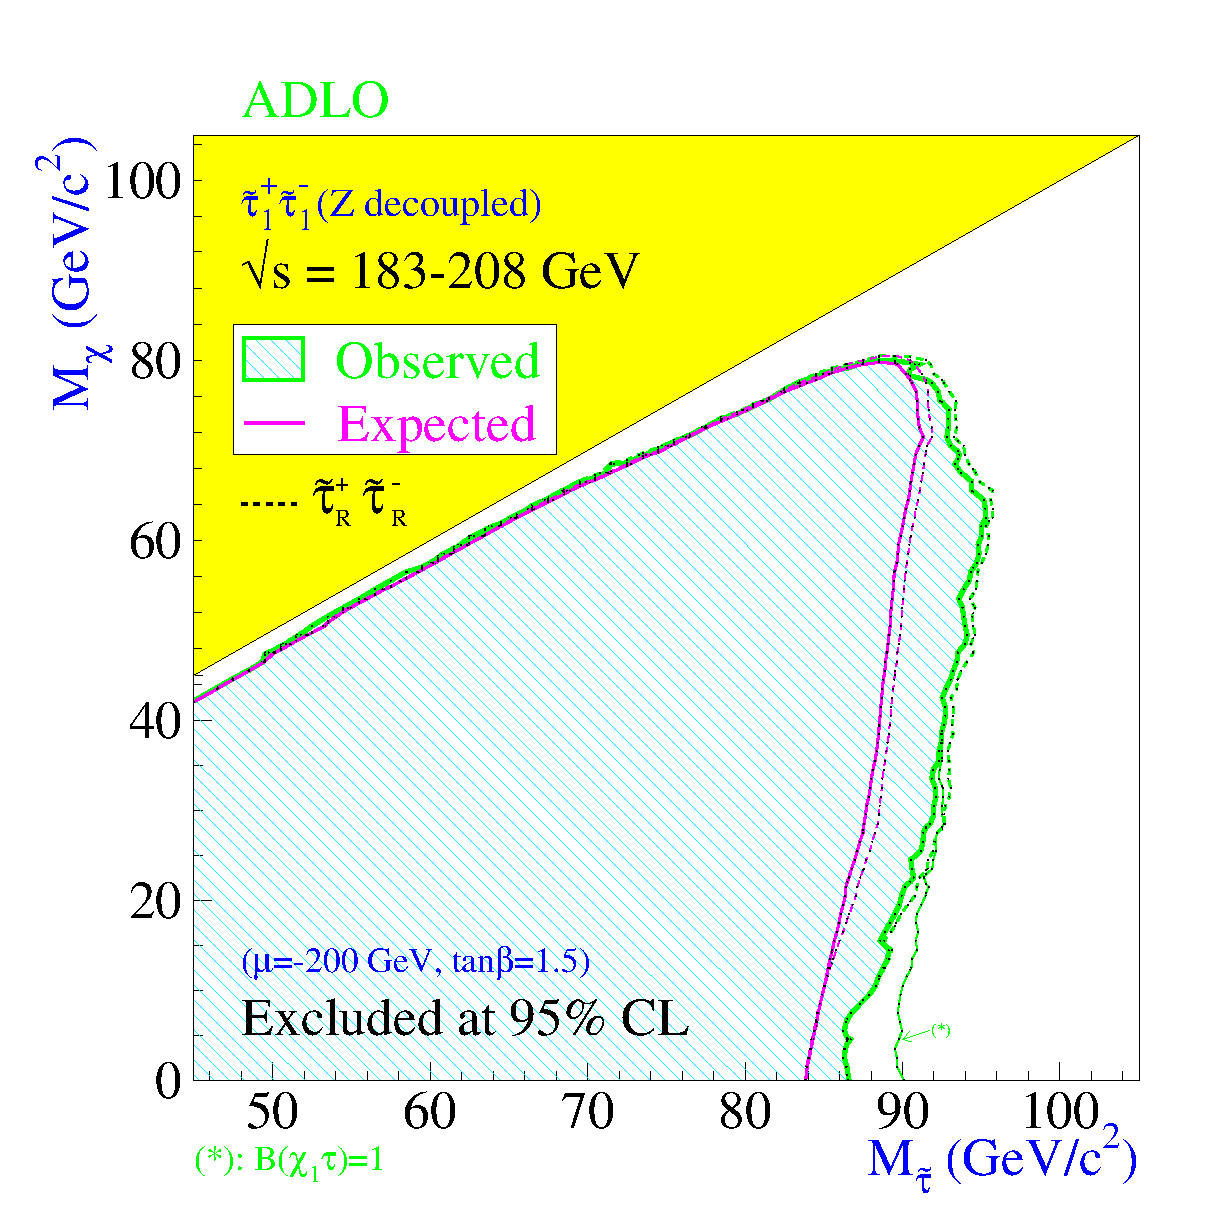
\includegraphics[width=0.7\linewidth]{figs/lep_stau}
 \caption{Expected and observed exclusion limits in the \textit{stau mass - neutralino mass} plane. The braching ratio for right-handed stau decaying to tau lepton + $\tilde{\chi}_1^0$ is included. The results were obtained by combining LEP data collected at center-of-mass energies ranging from 183 GeV to 208 GeV~\cite{lep:stau}.}
 \label{fig:lepstau}
\end{figure}

At the CERN LHC, 
the ATLAS~\cite{Aad:2014yka, Aad:2015eda} and 
CMS~\cite{Khachatryan:2016trj, Khachatryan:2015kxa, Sirunyan:2018vig}
collaborations have both performed searches for direct and indirect stau production with 8 TeV and 13 TeV center-of-mass energy LHC data.  The CMS collaboration has reported for a degenerate production scenario, in which both left- and right-handed $\tilde{\tau}$ pairs are produced, exclusions of $\tilde{\tau}$ masses up to 150 GeV when assuming a nearly massless neutralino~\cite{CMS-PAS-SUS-18-006}.
The ATLAS Collaboration has shown results of a search for SUSY in final states with $\tau$ leptons, probing indirect $\tilde{\tau}$ production in models of chargino-neutralino and chargino pair production, using data collected at $\sqrt{s} = 13$~TeV~\cite{Aaboud:2017nhr, Aad:2019byo}. Finally, ATLAS  released in 2019 results of the indirect stau search analysis showing the  first results on upper limits on the $\tilde{\tau}$ production cross-section excluding stau masses from 120~GeV to 390~GeV and a massless lightest neutralino~\cite{ATLAS-CONF-2019-018}. 

The search for stau-pairs is very challenging predominantly due to the low production cross section as an electroweak process in hadron collisions (see Figure~\ref{fig:xsec1}). Despite this fact, complex cut-and-count and machine learning techniques are developed to maximize the  sensitivity for scenarios involving the direct production of stau pairs, as well as their indirect production via the decays of charginos and neutralinos.  In this thesis, simplified SUSY models~\cite{PhysRevD.79.075020, PhysRevD.79.015005, Alves_2012} are examined, in which the $\tilde{\tau}$ can be produced directly through pair production, as shown in Figure~\ref{fig:staustau-tautaun1n1}.
The lightest neutralino is the LSP and purely bino, and the two charged staus are assumed to be mass-degenerated. The left- and right-handed staus are assumed to decay with a 100\% branching fraction to a bino-like neutralino, $\tilde{\tau}^\pm_{\mathrm{L},\;\mathrm{R}}  \to \tau^\pm\; \tilde{\chi}_1^0$, whereas all sparticles other than those explicitly mentioned here are assumed to be inaccessible at the LHC energy.
%Furthermore, the search considers final states with two hadronically decaying tau leptons stemming from the $\tilde{\tau}$-pair  decay to two  $\tau$ leptons and two $\tilde{\chi}_1^0$.


\subsection{Methodology}

This first ATLAS stau search with LHC Run2 data targets the direct production of a pair of staus, each decaying into one tau lepton and one invisible LSP. Each tau lepton stemming from the $\tilde{\tau}$ decay undergoes a subsequent decay into hadrons ($\tau \to \text{hadrons}\,\, \nu_\tau$) and an invisible neutrino. Signal events would thus be characterized by the presence of two sets of close-by hadrons and large missing transverse energy originating from the escaping invisible LSP and neutrinos.

Orthogonal signal regions (SR) were optimized for stau discovery by varying the kinematic selection criteria. 
Events are required to have have exactly two tau candidates with opposite-sign electric charge (OS). They are selected by the asymmetric di-tau trigger to cover the low stau mass region ($75~\text{GeV}<E_\mathrm{T}^\mathrm{miss}<150$~GeV) and by the 
di-tau +$E_\mathrm{T}^\mathrm{miss}$ trigger to cover the high stau mass region ($E_\mathrm{T}^\mathrm{miss}>150$~GeV).

The main background contributing to the selected final states are SM processes from QCD multijet, W+jets and diboson production.
Background events may contain a combination of `real' tau leptons, defined as correctly identified prompt
tau leptons, or `fake' tau leptons, which can originate from a misidentified quark or gluon jet, an electron, or a muon.  Smaller SM backgrounds arise from Z+jets production, or events that
contain a top quark or a top-quark pair in association with jets or additional W or Z bosons.
To estimate these irreducible background contributions,  MC simulated samples are used and validated in dedicated validation regions. Other SM backgrounds are found to be negligible.

One of the dominant backgrounds in the SRs originates from jets misidentified as tau leptons in multijet
production, where  nearly all hadronically decaying tau candidates are misidentified jets.
The multijet contribution in the SRs is estimated from data using the so-called ABCD method. 
This method defines various non-overlapping regions in a two-dimensional plane, as a function of two (or more) discriminating variables that are largely uncorrelated. More specifically, events are classified in regions differing by the product of electric charge of the tau-pair and the identification requirements of the tau candidates, either loose or tight. These regions are also constructing for varying cuts on the discriminating observables $E_\mathrm{T}^\mathrm{miss}$ or $m_{\mathrm{T}2}$ (see definition in Equation~\ref{eq:mt2}). The number of multijet events in the search region with OS tau-lepton pairs can therefore be calculated from  multijet events in regions identified with tau-lepton pairs having same sign of electric charge (SS) and passing the tight requirements of the tau identification. 
Afterwards, a transfer factor, which is extracted in regions where the tau candidates pass only the loose identification requirements, is used to provide the correct normalization of the multijet estimate.
This transfer factor is defined as the ratio between the number of events with OS tau pairs to the number of events with SS tau-pair candidates.


The multijet background estimation is also validated using a different method, the \textit{fake-factor} method. Fake factors (FF) are derived for each of the two tau candidates with the same electric charge in a multijet enriched region. They are computed as the ratio of the number of leading or subleading tau candidates passing all of the nominal signal identification criteria over the number of tau candidates failing the requirement on the tau identification, and are parameterized with respect to the $p_T$, $\eta$ and number of tracks of the tau candidates. The expected number of multijet events entering a selection is computed by applying the fake factors to the yields in a set of sideband regions where either the leading, subleading or both tau candidates fail the identification requirements. Agreement of the predicted multijet event yields from the ABCD method and the FF method is observed within the statistical and systematic uncertainties.


The production of W+jets events with at least one misidentified tau lepton is an important background,
accounting for about 25\% of the expected SM background in the two SRs. It is  estimated from MC simulation and normalized to data in a dedicated control region.

Systematic uncertainties have an impact on the estimates of the background and signal event yields in the
signal regions. Uncertainties arising from experimental and theoretical sources are estimated in the analysis and considered in the statistical analysis to interpret the results. 
The main sources of experimental systematic uncertainty in the SM background estimates include tau lepton and jet energy scale and resolution, tau lepton identification, pile-up, and uncertainties related to the
modelling of $E_\mathrm{T}^\text{miss}$ in the simulation. 
Uncertainties arising from ABCD method to determine the QCD multijet events are also considered, dominated by the the correlation between the tau identification, the charge requirement, and the kinematic variable $m_{\mathrm{T}2}$.
Finally, theoretical uncertainties affecting the MC event generator predictions, for the W+jets, Z+jets
and multi-boson samples, are estimated by varying the renormalisation and factorisation scale as well as
PDF uncertainties. The dominant uncertainties in the SRs are tau identification and energy scale (14 - 29\%) and the statistical uncertainty of the signal MC predictions (6 - 10\%). The multijet
normalization with respect to the prediction from the ABCD method in the SR has an uncertainty
of around 30\%, due to the small number of observed events in the multijet regions.
The cross-section uncertainty is taken into account as main source of signal modeling theoretical uncertainty, and it varies from 3\% to 7\% for the considered SUSY models.


\subsection{Results}

Selected events are distributed according to the $m_{\mathrm{T}2}$ observable for data, expected SM backgrounds, and the SUSY signal models.  In both signal regions of the analysis, observations and background predictions are found to be compatible within uncertainties.

In the absence of a significant excess over the expected SM background, the observed and expected numbers
of events in the signal regions are used to place exclusion limits at 95\% CL using the model-dependent limit fit. The exclusion limits for the combined low-mass and high-mass SRs for the simplified models described previously are shown in Figure~\ref{fig:stau1}.
\begin{figure}
 \centering
 \includegraphics[width=0.7\linewidth]{figs/stau1}
 \caption{The 95\% CL exclusion contours for the combined fit of low-mass and high-mass signal regions for simplified models with combined production. The solid (dashed) lines show the observed (expected) exclusion contours. The band around the expected limit shows the $\pm 1~\sigma$ variations, including all uncertainties except theoretical uncertainties in the signal cross section. The dotted lines around the observed limit indicate  the sensitivity to $\pm 1~\sigma$ variations of the theoretical uncertainties in the signal cross section~\cite{ATLAS-CONF-2019-018, Aad:2019byo}.}
 \label{fig:stau1}
\end{figure}
While the left-handed stau pair production has a higher production cross section, the right-handed stau pair production has a higher efficiency times acceptance due to kinematic differences in the resulting decay products. Stau masses from 120 GeV to 390 GeV are excluded for a massless lightest neutralino in the scenario of the combined left- and right-handed stau-pair production.

These limits significantly extend previous results~\cite{Aad:2015eda, Khachatryan:2014qwa, Sirunyan:2018vig} in the high $\tilde{\tau}$ mass region.

\subsection{Conclusions}
Searches for stau-pair production in events with at least two hadronically decaying $\tau$-leptons and missing
transverse momentum were performed using $139~\mathrm{fb}^{-1}$ of $pp$ collision data at $\sqrt{s} = 13$~TeV recorded with
the ATLAS detector at the LHC~\cite{ATLAS-CONF-2019-018, Aad:2019byo}.
Agreement between data and SM predictions is observed in the optimized
signal regions. The results are used to set limits on the visible cross section for events beyond the SM in each signal region.
Exclusion limits are placed on parameters of simplified electroweak supersymmetry models in scenarios of stau-pair production. Stau masses from 120 GeV to 390 GeV are excluded for a massless lightest neutralino
in the scenario of direct production of stau pairs, with each stau decaying into the lightest neutralino and one $\tau$-lepton. These limits extend significantly beyond previous results by the ATLAS and CMS experiments
in the high stau mass region.

\chapter{Synopsis}

\section{Summary}

The search of SUSY is an important part of the physics program at CERN's LHC. The large amount of data successfully collected by the experiments so far, provide a unique opportunity to explore SUSY with novel analysis techniques.

If particles predicted by SUSY exist and are not extremely massive, they must be produced at LHC collision events and could be hiding in data collected by the ATLAS and CMS detectors. However, unlike most processes at the LHC, which are governed by strong force interactions, electroweak superpartners would be created through the much weaker electroweak interaction, thus lowering their production rates. Further, most of these new SUSY particles are expected to be unstable and can be searched by tracing their decay products -- typically into a known  SM particle and a \textit{LSP}, which could be stable and non-interacting, thus forming a natural dark matter candidate. 

Despite the low production cross-section of electroweak SUSY processes, events with many leptons in the final state are very interesting since SM processes mimicking them are very rare.
ATLAS searched for such multi-lepton events and presented the results in terms of the number of events from new physics processes with a four-lepton signature, and also in terms of RPV and RPC SUSY models.  All data yields are found to be consistent with  SM expectations and results are thus used to set upper limits on the event yields from processes beyond the   SM. 
Stringent exclusion limits are set in simplified models of
GGM SUSY with higgsino particles, which are assumed to decay into either Higgs or Z bosons.  In RPV simplified models with decays of the LSP to charged leptons, exclusions are placed on the mass of wino, slepton and gluino masses up to the TeV scale, extending significantly the lower limit results set by previous ATLAS searches.
 

Until recently, an important superpartner of the tau slepton, the "stau", had yet to be searched for beyond the exclusion limit of around 90 GeV found at the LHC's predecessor at CERN, the LEP collider. 
A light stau, if it exists, could play a role in neutralino co-annihilation, moderating the amount of dark matter in the visible universe, which otherwise would be too abundant to explain astrophysical measurements. The search for a light stau is experimentally challenging due to its extremely low production rate in LHC $pp$ collisions, requiring advanced techniques to reconstruct the  SM tau leptons it can decay into. In fact, during the LHC Run 1 data taking period, only a narrow parameter region around a stau mass of 109 GeV and a massless lightest neutralino could be excluded by LHC experiments~\cite{Aad:2015eda}. 
In LHC Run 2, ATLAS search efforts target the direct production of a pair of staus, each decaying into one tau lepton and one invisible LSP.  The ATLAS data do not reveal hints for stau pair production and thus new exclusion limits are set on the mass of staus using different assumptions on the presence of both possible stau types (left and right, referring to the two different spin states of the tau partner lepton). The limits obtained supersede significantly the LEP results and are in fact the strongest obtained so far in collider experiments.

Overall, both sets of results place strong constraints on important supersymmetric scenarios, which will guide future ATLAS searches. Further, they illustrate the benefits brought by advanced analysis techniques, which help improve the sensitivity to new physics phenomena at colliders in the future.

\section{Outlook}

The absence of any observation of new phenomena at the first run of the LHC
at $7,\, 8,\, 13$~TeV place significant constraints on SUSY parameter space. 
As displayed in Figure~\ref{fig:susysum}, inclusive searches probe production of gluinos at about 2.2 TeV, 
first and second generation squarks in the range of about 1 to 1.8 TeV, 
third generation squarks at scales around 600 GeV to 1 TeV,
electroweak gauginos at scales around 300 to 800 GeV, and sleptons up to 800 GeV. 
However, depending on the assumptions made on the underlying SUSY spectrum these limits can also weaken considerably.
\begin{sidewaysfigure}
%\begin{figure}
	\centering
	\includegraphics[width=0.99\linewidth]{figs/susysum}
	\caption{Mass reach of the ATLAS searches for SUSY. Results are quoted for the nominal cross section in both a region of near-maximal mass reach and a demonstrative alternative scenario, in order to display the range in model space of search sensitivity. Some limits depend on additional assumptions on the mass of the intermediate states, as described in the references provided in the plot. In some cases these additional dependencies are indicated by darker bands showing different model parameters~\cite{ATL-PHYS-PUB-2019-022}.}
	\label{fig:susysum}
%\end{figure}
\end{sidewaysfigure}

With the LHC having reached almost its maximum energy of $\sqrt{s} = 14$~TeV, future sensitivity increase in searching for SUSY will have to originate from higher data statistics, the evolution of the trigger and improvement of experimental analysis techniques, since there will be no significant proton beam energy increase anymore.
Therefore, it is expected that the current landscape of SUSY searches and corresponding exclusion limits at the LHC,  as that shown in Figure~\ref{fig:susysum} from the ATLAS experiment~\cite{ATL-PHYS-PUB-2019-022}, will not change as rapidly anymore as it did in the past, when the LHC underwent several successive increases of collision energy.

The ongoing LHC run at $\sqrt{s} = 13$ TeV, and future runs at 14 TeV with significantly larger integrated luminosities (Run 3, and the High-Luminosity LHC), will provide a large data sample for future SUSY searches. Although the sensitivity for colored sparticles is expected to increase, the expanded data set will be particularly beneficial for electroweak gaugino searches, and for the more difficult final states presented by compressed particle spectra, long-lived sparticles, and RPV scenarios.

\newpage
%$\text{TE\Lambda O\Sigma \quad KAI\quad T \Omega \quad TPIA\Delta IK\Omega \quad \Theta E\Omega \Delta O \Xi A}$

\vspace*{\fill}
\begin{center} 
	$\mathrm{ TE\Lambda O \Sigma\quad KAI \quad T\Omega \quad TPIA\Delta IK\Omega \quad \Theta E \Omega \quad \Delta O\Xi A, \; TIMH \quad KAI \quad \Pi PO \Sigma KYNH\Sigma I \Sigma}$
\end{center}

\iffalse
\fi

\chapter*{References}
%\nocite{*}
\printbibliography[heading=none]

\chapter{Appendix}\label{ch:app}

Papers published at scientific journals, including the work of this thesis, are accumulated in this section.

\end{document}